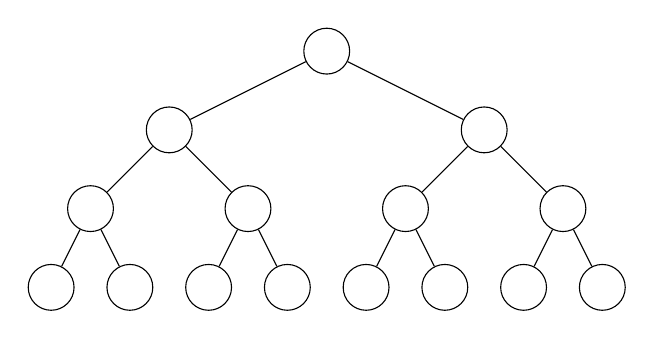
\begin{tikzpicture}[level distance=10mm]
  \tikzstyle{every node}=[circle,text width=0.3cm]
  \tikzstyle{level 1}=[sibling distance=4cm]
  \tikzstyle{level 2}=[sibling distance=2cm]
  \tikzstyle{level 3}=[sibling distance=1cm]
  \node[circle,draw] {} 
  child{node[circle,draw]{} 
    child{node[circle,draw]{} 
      child{node[circle,draw]{}}
      child{node[circle,draw]{}}
    }
    child{node[circle,draw]{} 
      child{node[circle,draw]{}}
      child{node[circle,draw]{}}
    }
  }
  child{node[circle,draw]{} 
    child{node[circle,draw]{} 
      child{node[circle,draw]{}}
      child{node[circle,draw]{}}
    }
    child{node[circle,draw]{} 
      child{node[circle,draw]{}}
      child{node[circle,draw]{}}
    }
  };

\end{tikzpicture}
